\section{An Explanation of the Grokking Phenomenon}
\label{sec:explanation}

In this section, we provide an explanation of the grokking phenomenon based on~\cite{KumarBGP24}, which claims that grokking happens as a transition between different regimes of training.
We first briefly review the kernel regime and rich regime defined in~\cite{KumarBGP24} in \cref{subsec:regimes}, and illustrate how they help explain the grokking phenomenon for modular addition in \cref{subsec:explain_by_regimes}.

\subsection{Kernel Regime And Rich Regime}
\label{subsec:regimes}

We have the following definition of neural tangent kernel (NTK).

\begin{definition}[Neural Tangent Kernel~\cite{JacotHG18,KumarBGP24}]
    \label{def:NTK}
    Let $\Theta$ be the parameter space and $\mathcal{X}$ be the input space.
    Let $f \colon \Theta \times \mathcal{X} \to \mathcal{Y}$ be a neural network.
    For $\theta \in \Theta$, the \emph{neural tangent kernel} of $f(\theta, \cdot)$ is defined as 
    \begin{align*}
        K_\theta(\mathbf{x}, \mathbf{x}') := \nabla_\theta f(\theta, \mathbf{x}) \nabla_\theta f(\theta, \mathbf{x}')^\top, 
        \quad \forall \mathbf{x}, \mathbf{x}' \in \mathcal{X}.
    \end{align*}
\end{definition}

In the \emph{kernel regime}, we have the following approximation of the model output, 
\begin{align*}
    f(\theta, \mathbf{x}) \approx f(\theta_0, \mathbf{x}) + \Braket{\nabla_{\theta} f(\theta_0, \mathbf{x}), \theta - \theta_0}.
\end{align*}
Note that the right-hand side is linear in $\theta$, which means that $f(\theta, \cdot)$ has approximately the same expressivity as the kernel method with respect to $K_{\theta_0}$, as defined in \cref{def:NTK}.
Under gradient descent, the model's parameters $\theta$ are restricted to the affine subspace $W := \mathrm{span}\{\nabla_{\theta} f(\theta_0, \mathbf{x}_i)\}_{i=1}^n$.
Therefore, the model will first converge to the local optimal solution $\theta_W^* \in W$ in the kernel regime.
\emph{This corresponds to the stage where the model overfits the training data but does not generalize.}

When the model begins to learn important non-linear features, it will escape $W$ and enter the \emph{rich regime}, where it finally converges towards the global optimal solution $\theta^*$.
\emph{This corresponds to the generalization phase in the grokking phenomenon.}

It is worth mentioning that normalization methods such as weight decay accelerates generalization by encouraging the model to escape from the kernel regime, which is consistent with our experiment results in \cref{sec:subtask3}.


\subsection{Regime Transition in Modular Addition Problem}
\label{subsec:explain_by_regimes}

We further illustrate how grokking is related to the transition between the aforementioned two regimes in the modular addition problem.
We first rewrite the target function $f^*$ as 
\begin{align*}
    f^*(e_a, e_b) = e_{a+b} = H^a e_b = H^b e_a, 
\end{align*}
where $H = \sum_{j=0}^{p-1} e_{j+1} e_{j}^\top$ is the $p \times p$ cyclic permutation matrix.
When the first (second) coordinate of $f^*$ is fixed, it becomes a simple linear function of the second (first) coordinate.
Following this observation, we consider the following generalized version of $f^*$.

Let $A$ be any non-empty subset of $\ZZ_p$, and $E(A) := \{e_a \colon a \in A\}$. Denote $E(\ZZ_p) := \{e_0, e_1, \dots, e_{p-1}\}$.
Define $f_A^* \colon E(A) \times E(\ZZ_p) \to E(\ZZ_p)$ to be the restriction of $f^*$ on $E(A) \times E(\ZZ_p)$.
Intuitively, the smaller $\norm{A}$ is, the closer $f_A^*$ is to a linear map.
We define $\lambda := \frac{\norm{A}}{p} \in (0, 1]$ to be a measure of the ``non-linearity'' of $f_A^*$.
Specifically, $f^* = f_{\ZZ_p}^*$, and thus has non-linearity $1$.

To prove the explanations in \cref{subsec:regimes}, we study how the non-linearity $\lambda$ influences the grokking phenomenon.
For each given $\lambda$, we sample a random subset $A \subseteq \ZZ_p$ of size $\lambda p$.
We then train a $2$-layer MLP on $A \times \ZZ_p$ with training data fraction $\alpha = 0.6$, SGD optimizer and weight decay $0$ to learn the target function $f_A^*$.
The results are shown in \cref{fig:acc_and_loss_different_lambda}.

\begin{figure}[!ht]
    \centering
    \begin{subfigure}{0.45\textwidth}
        \centering
        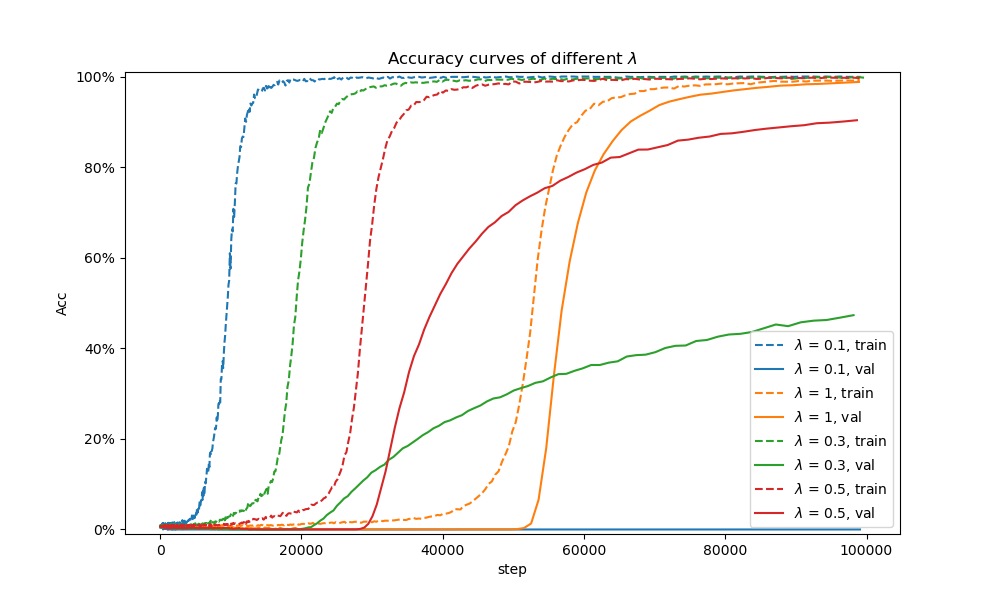
\includegraphics[width=\linewidth]{fig/grokking_curves/different_Afraction_acc.png}
        \caption{Training and validation accuracy}
        \label{fig:different_lambda_acc}
    \end{subfigure}
    %\hfill
    \begin{subfigure}{0.45\textwidth}
        \centering
        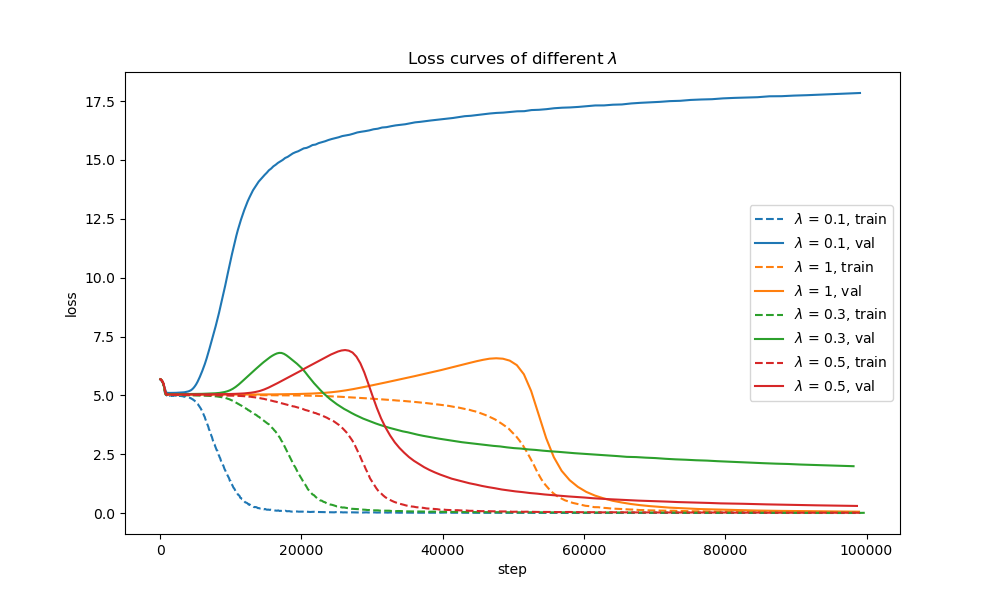
\includegraphics[width=\linewidth]{fig/loss_curves/different_Afraction_loss.png}
        \caption{Training and validation loss}
        \label{fig:different_lambda_loss}
    \end{subfigure}

    \caption{Learning curves of different target functions $f_A^*$.}
    \label{fig:acc_and_loss_different_lambda}
\end{figure}

\cref{fig:different_lambda_acc} shows that it becomes slower to overfit the training data as non-linearity $\lambda$ increases.
Perhaps surprisingly, generalization nevertheless becomes easier as $\lambda$ increases.
For $\lambda = 0.1$, the model does not generalize at all and the validation loss blows up.
For $\lambda = 0.3$ and $0.5$, some generalization happens, but the validation loss does not fully converge within $10^5$ steps.
For $\lambda = 1.0$, the model quickly generalizes after it begins to fit the training data, and the grokking phenomenon almost vanishes.

We believe this interesting result reflects the mechanism of regime transition.
For smaller $\lambda$'s, the target function $f_A^*$ behaves more like a linear function.
Hence, the model tends to first learn these linear features.
It is then trapped in the kernel regime, and have to take a long time to escape from the affine subspace $W$ and enter the rich regime;
this is how grokking happens.
To be specific, the peaks of the loss curves in \cref{fig:different_lambda_loss} approximately corresponds to the kernel regime, and the similar shapes can also be observed in \cref{fig:loss_curve_transformer,fig:loss_curve_LSTM,fig:loss_curve_MLP}.
In contrast, For a larger $\lambda$, the function $f_A^*$ is very far from a linear map, hence forcing the model to learn other useful features.
Therefore, the model quickly moves to the rich regime and converges to the global optimal solution.
Since the transition happens immediately, grokking almost disappears in this setting.